\documentclass{beamer}

\mode<presentation>
{
  \usetheme{CambridgeUS}      % or try Darmstadt, Madrid, Warsaw, ...
  \usecolortheme{default} % or try albatross, beaver, crane, ...
  \usefonttheme{default}  % or try serif, structurebold, ...
  \setbeamertemplate{navigation symbols}{}
  \setbeamertemplate{caption}[numbered]
} 

\usepackage[english]{babel}
\usepackage[utf8x]{inputenc}

\title[Efficiently Inefficient]{Chapter 9: Quantitative Equity Investing}

\author{Chi Ma\\}

\institute{\bf Qishi Buyside StudyGroup}
%\textsc {Industrial Training Presentation }

\date{$30^{\text{th}}$ Nov 2019}

\begin{document}

\begin{frame}
  \titlepage
\end{frame}
\tableofcontents

\section{Fundamental Quantitative Investing}

\begin{frame}{Fundamental Quantitative Investing}

\begin{itemize}
  \item OLTAS is a private owned product used by Yes Bank.
  \item A system which can integrate with internet portal and provide facility of making tax payments to their end internet portal users.
\end{itemize}

% Commands to include a figure:
\begin{figure}
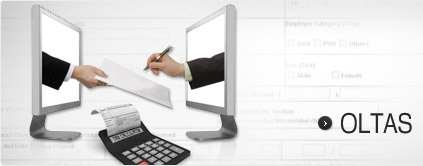
\includegraphics[width=5cm ,height= 3cm]{oltas-header.jpg}
\caption{\label{fig:your-figure}OLTAS}
\end{figure}
\vskip 1cm

\end{frame}
%%%%%%%%%%%%%%%


\section{Statistical Arbitrage}

\begin{frame}{MySpace}

\begin{itemize}
  \item OLTAS is a part of MySpace.
  \item MySpace is totally for customer’s space, where different types of services like insurance schemes , cheque printing, online payments, gifts and voucher offers provided by Yes Bank under one application.

\end{itemize}

% Commands to include a figure:
\begin{figure}

\includegraphics[width=5cm ,height= 3cm]{multitasking_cartoon.jpg}
\caption{\label{fig:your-figure}MySpace}
\end{figure}
\vskip 1cm

\end{frame}

%%%%%%%%%%%%%%%

\section{HFT}

\begin{frame}{Yes Bank and NSDL}

\begin{itemize}
  \item Yes Bank is a depository participant of NSDL.

  \item Yes Bank act as a middle man in the process of online tax payment.

\end{itemize}

\vskip 1cm
\end{frame}

\begin{frame}{NSDL}

\begin{itemize}
  \item NSDL is promoted byIndustrial Development Bank of India Limited(IDBI) - the largest development bank of India.
\item NSDLis an Indian central securities depository.

\end{itemize}
\vskip 1cm

\end{frame}


%%%%%%%%%%%%%%%%

\section{Interview with Asness}

\begin{frame}{Benefits}

\begin{block}{From customer’s point of view}
\end{block}
\begin{itemize}

%\end{}{itemize}
\item Ease of access : Tax payers can track online the status of their challans deposited in banks
\item Secure
  \item Check present status of challan
  \item Get Confirmation

\end{itemize}

\begin{block}{From Bank’s point of view}
\end{block}
\begin{itemize}

%\end{}{itemize}
\item Provide multiple services
\item Make Business
\item Increase Brand Value
\end{itemize}

\vskip 1cm
\end{frame}

%---------------------


\end{document}
